\documentclass[12pt,a4paper]{article}
\usepackage{iftex}
\ifPDFTeX
  \usepackage[T2A]{fontenc}\usepackage[utf8]{inputenc}
\else
  \usepackage{fontspec}
  \setmainfont{Liberation Serif}
  \setsansfont{Noto Sans}
  \setmonofont{DejaVu Sans Mono}[Scale=0.80]
\fi
\usepackage[ukrainian]{babel}
\usepackage[a4paper,left=23mm,right=22mm,top=23mm,bottom=24mm]{geometry}
\usepackage{microtype,setspace,graphicx,array,longtable,tabularx,booktabs}
\usepackage{enumitem,xcolor,tcolorbox,float,caption,fancyhdr,titlesec}
\usepackage{hyperref,url,lastpage,ragged2e,listings}
\setstretch{1.15}\setlength{\emergencystretch}{3em}
\graphicspath{{screenshots/}}
\newcommand{\AuthorName}{Суворов Дмитро}
\newcommand{\StudentGroup}{ЦІ-31}
\definecolor{forest}{HTML}{233C30}\definecolor{sage}{HTML}{5B7957}
\definecolor{mist}{HTML}{F0F4EE}\definecolor{rulegray}{HTML}{D9E1DA}
\definecolor{codebg}{HTML}{F5F7F5}
\hypersetup{hypertexnames=false,colorlinks=true,linkcolor=forest,urlcolor=sage,pdftitle={Звіт КП №3 — тестування Ритм},pdfauthor={Суворов Дмитро}}
\titleformat{\section}{\Large\sffamily\bfseries\color{forest}}{\thesection.}{0.6em}{}
\titleformat{\subsection}{\large\sffamily\bfseries\color{forest}}{\thesubsection.}{0.6em}{}
\titlespacing*{\section}{0pt}{15pt}{8pt}\titlespacing*{\subsection}{0pt}{11pt}{5pt}
\captionsetup{font=small,labelfont={bf,color=forest},justification=centering}
\setlist[itemize]{leftmargin=1.45em,itemsep=2pt,topsep=4pt}
\setlist[enumerate]{leftmargin=1.55em,itemsep=2pt,topsep=4pt}
\renewcommand{\arraystretch}{1.18}
\pagestyle{fancy}\fancyhf{}
\fancyhead[L]{\small\sffamily\color{sage} КП №3 · Тестування ПЗ}
\fancyhead[R]{\small\sffamily\color{sage} Ритм}
\fancyfoot[L]{\footnotesize\color{sage} \AuthorName\ · 2026}
\fancyfoot[R]{\footnotesize\color{sage} \thepage\,/\,\pageref{LastPage}}
\renewcommand{\headrulewidth}{0.4pt}\setlength{\headheight}{26pt}
\newtcolorbox{infobox}{colback=mist,colframe=rulegray,boxrule=0.5pt,arc=2mm,left=3mm,right=3mm,top=2mm,bottom=2mm}
\lstset{basicstyle=\ttfamily\footnotesize,backgroundcolor=\color{codebg},frame=single,rulecolor=\color{rulegray},breaklines=true,showstringspaces=false,columns=fullflexible,xleftmargin=2mm,xrightmargin=2mm,aboveskip=5pt,belowskip=5pt}
\newcommand{\file}[1]{\path{#1}}

\begin{document}
\begin{titlepage}\thispagestyle{empty}\centering
{\small\sffamily\bfseries МІНІСТЕРСТВО ОСВІТИ І НАУКИ УКРАЇНИ}\par\vspace{5mm}
{\small\sffamily\bfseries НАЦІОНАЛЬНИЙ ТЕХНІЧНИЙ УНІВЕРСИТЕТ УКРАЇНИ}\par
{\small\sffamily\bfseries «КИЇВСЬКИЙ ПОЛІТЕХНІЧНИЙ ІНСТИТУТ ІМЕНІ ІГОРЯ СІКОРСЬКОГО»}\par
\vspace{30mm}{\LARGE\sffamily\bfseries\color{forest} ЗВІТ}\par\vspace{7mm}
{\Large Комп'ютерний практикум №3}\par\vspace{5mm}
{\large «Тестування програмного забезпечення»}\par\vspace{12mm}
з дисципліни\par\medskip
{\large\bfseries «Технології розробки WEB-орієнтованих систем»}\par\vspace{15mm}
\begin{infobox}\centering\large\bfseries Тема №69: «Спортзал»\\Web-застосунок «Ритм»\end{infobox}
\vfill\begin{flushright}Виконавець: \textbf{\AuthorName}\\Група: \StudentGroup\\Викладач: С. В. Суліма\end{flushright}\vfill
Київ --- 2026
\end{titlepage}
\tableofcontents\clearpage

\section{Мета та виконані завдання}
Мета роботи --- спланувати й провести комплексне ручне та автоматизоване тестування наскрізного web-проєкту «Ритм», задокументувати дефекти, виконати виправлення і регресію.
\begin{itemize}
\item складено тест-план з областю, стратегією, ризиками та критеріями завершення;
\item виконано 9 ручних позитивних і негативних тест-кейсів;
\item реалізовано 12 unit-тестів бізнес-правил та валідації;
\item реалізовано 12 інтеграційних REST API-тестів із реальною PostgreSQL;
\item зафіксовано 3 дефекти, виконано виправлення та повну регресію;
\item одна команда \file{npm test} формує результат і звіт V8 coverage.
\end{itemize}
\noindent\begin{tabularx}{\textwidth}{>{\bfseries}p{40mm}X}
Виконавець & \AuthorName\\Група & \StudentGroup\\
Внесок & Планування, ручні кейси, unit/API-автоматизація, аналіз дефектів, виправлення, регресія і документація\\
\end{tabularx}

\section{Тест-план}
\subsection{Об'єкти та область}
Перевірялися сім клієнтських сторінок, форми реєстрації/входу/запису, каталог, кабінет, адміністративний CRUD, маршрути \file{/api/auth}, \file{/api/trainings}, \file{/api/bookings}, \file{/api/categories}, \file{/api/health}, ролі member/admin, ізоляція власника та обмеження PostgreSQL.

Поза областю залишено production-навантаження, платіжні та зовнішні інтеграції, яких у застосунку немає.

\subsection{Стратегія}
\begin{enumerate}
\item Ручне функціональне тестування «чорної скриньки»: позитивні, негативні та межові сценарії у Chromium.
\item Unit-тестування «білої скриньки»: чисті функції та Zod-схеми модуля \file{server/validation.js} через \file{node:test}.
\item Інтеграційне API-тестування: Supertest викликає реальний Express, запити виконуються у PostgreSQL 17, тимчасові дані видаляються після набору.
\item Security-перевірки: 401 без JWT, 403 для member, відсутність mass assignment ролі, bcrypt-межі пароля.
\item Повна регресія після виправлень командою \file{npm test} та повторенням ручних сценаріїв.
\end{enumerate}

\subsection{Середовище та критерії завершення}
Node.js 26.13.0, npm 12.2.2, Express 5, PostgreSQL 17.11 у Docker Compose, Chromium, Linux. Вихідні критерії: щонайменше 5 ручних, 5 unit і 5 API-тестів; 100\% Passed; відсутні відкриті Critical/Major; усі дефекти мають картки; сформовано coverage і test summary. Усі критерії виконано.

\section{Ручні тест-кейси}
Кожний кейс має ID, назву, передумови, кроки, очікуваний і фактичний результат та статус. Повні описи містяться у \file{docs/TEST-CASES.md}.
\begin{longtable}{>{\RaggedRight\arraybackslash}p{11mm}>{\RaggedRight\arraybackslash}p{45mm}>{\RaggedRight\arraybackslash}p{34mm}>{\RaggedRight\arraybackslash}p{31mm}>{\RaggedRight\arraybackslash}p{16mm}}
\toprule ID & Сценарій & Очікуваний результат & Фактичний результат & Статус\\\midrule
TC-01 & Реєстрація з коректними даними & 201, member, вхід & Створено, роль member & Passed\\
TC-02 & Слабкий пароль & 400, користувача немає & 400, поле password & Passed\\
TC-03 & Неправильний пароль & 401, токена немає & 401, спільне повідомлення & Passed\\
TC-04 & Створення запису & 201, дані у кабінеті/БД & Дані збігаються & Passed\\
TC-05 & Неправильний телефон & 400, запису немає & 400, поле phone & Passed\\
TC-06 & Часткове редагування & Інші поля збережені & Примітка збережена & Passed\\
TC-07 & Admin API від member & 403, без змін & 403 & Passed\\
TC-08 & CRUD тренування admin & 201/200/204/404 & Коди й дані коректні & Passed\\
TC-09 & Навігація desktop/mobile & Без 404/overflow & Усі сторінки доступні & Passed\\\bottomrule
\end{longtable}

\section{Автоматизовані unit-тести}
Unit-набір містить 12 тестів: межі PostgreSQL ID, normalizing email/імені, мінімальну довжину й bcrypt-межу 72 байти, strict-схему проти підміни ролі, валідні/минулі/неіснуючі дати, формат телефону, default примітки, тривалість і ціну тренування.
\begin{lstlisting}[caption={Приклад unit-тесту валідації ID}]
test("parseId rejects zero, fractions and injections", () => {
  for (const value of ["0", "1.5", "1 OR 1=1", "2147483648"])
    assert.throws(() => parseId(value), { status: 400 });
});
\end{lstlisting}
Модуль валідації винесено у \file{server/validation.js}; він не звертається до мережі/БД, тому тести швидкі та детерміновані.

\section{Автоматизовані REST API-тести}
Набір Supertest містить 12 сценаріїв: health, каталог, реєстрація, duplicate 409, неправильний пароль 401, захищений ресурс 401, validation 400, POST/PATCH/DELETE запису, 403 для member і JSON 404. Після прогону hook видаляє створені bookings/users.
\begin{lstlisting}[caption={Регресійний API-тест часткового оновлення}]
const response = await request(app)
  .patch(`/api/bookings/${bookingId}`)
  .set("Authorization", `Bearer ${token}`)
  .send({ phone: "+380671234567" })
  .expect(200);
assert.equal(response.body.data.note, "API regression");
\end{lstlisting}
Express app експортується без автоматичного відкриття порту; production-listener створюється лише при прямому запуску файлу.

\section{Запуск і покриття}
\begin{lstlisting}[caption={Єдина команда повної перевірки}]
docker compose up -d --wait db
npm run db:init
npm test
\end{lstlisting}
Результат: 24/24 автоматизованих тестів Passed. Загальне покриття: lines 80,44\%, branches 78,46\%, functions 67,57\%. Для \file{server/validation.js}: 100\% lines/branches/functions.
\begin{figure}[H]\centering
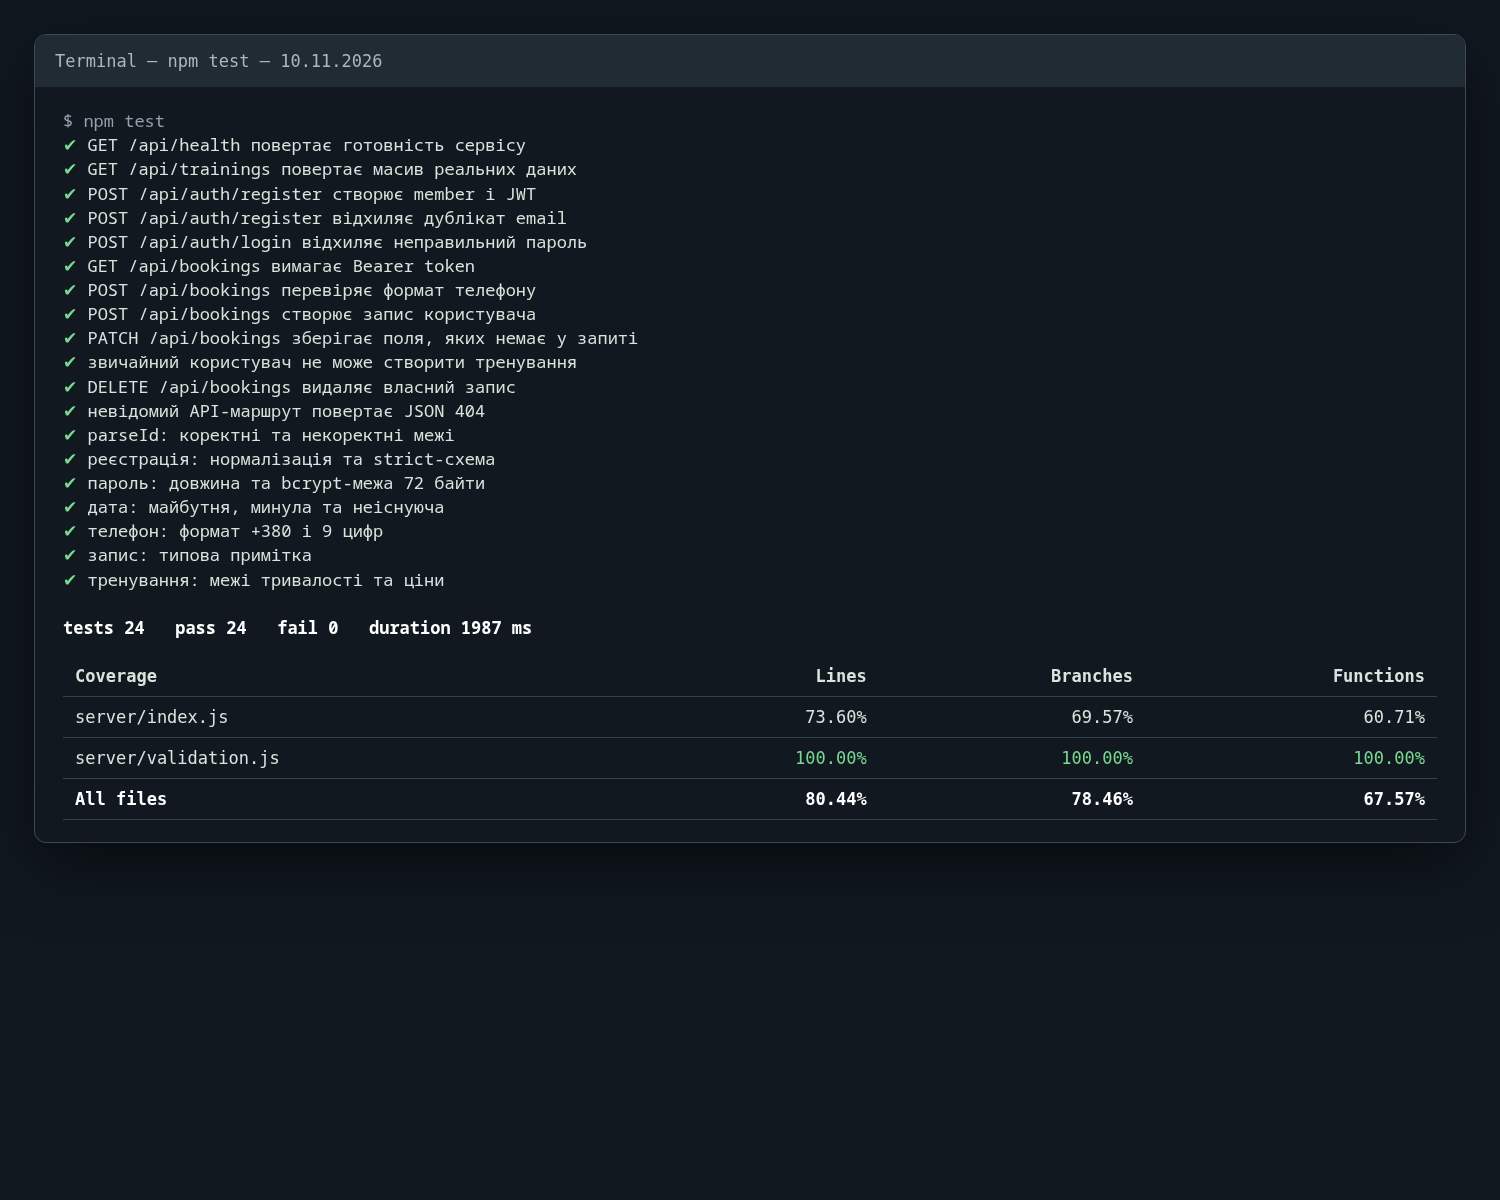
\includegraphics[width=\linewidth]{automated-tests.png}
\caption{Фактичний результат unit/API-тестів і coverage}
\end{figure}

\section{Баг-репорти та виправлення}
\subsection{BUG-001 --- PATCH стирав не передану примітку}
\textbf{Кроки:} створити запис із приміткою; PATCH лише телефону; повторно отримати запис. \textbf{Очікувано:} змінюється лише телефон. \textbf{Фактично до виправлення:} default у partial-схемі підставляв порожню примітку. \textbf{Критичність:} Major. \textbf{Виправлення:} для PATCH note є optional без default. \textbf{Статус:} Fixed/Verified автоматизованим regression-тестом.

\subsection{BUG-002 --- listener запускався при імпорті тестом}
\textbf{Кроки:} імпортувати Express app у Supertest при зайнятому порту. \textbf{Очікувано:} імпорт без мережевого listener. \textbf{Фактично:} можливий \file{EADDRINUSE}. \textbf{Критичність:} Major. \textbf{Виправлення:} експортовано \file{app}/\file{startServer()}, прямий запуск перевіряється окремо. \textbf{Статус:} Fixed/Verified 12 API-тестами.

\subsection{BUG-003 --- неактуальна команда PostgreSQL}
\textbf{Кроки:} виконати psql з \file{gym_user/gym_db}. \textbf{Очікувано:} консоль БД. \textbf{Фактично:} role does not exist. \textbf{Критичність:} Minor. \textbf{Виправлення:} README використовує \file{ritm/ritm}, додано SQL та troubleshooting. \textbf{Статус:} Fixed/Verified.

Усі дефекти оформлено окремими задачами GitHub і додано до дошки. Повний шаблон баг-репортів: \file{docs/BUG-REPORTS.md}.

\section{Підсумковий звіт}
\begin{center}\begin{tabular}{lrrrr}
\toprule Набір & Всього & Passed & Failed & Успішність\\\midrule
Ручні & 9 & 9 & 0 & 100\%\\
Unit & 12 & 12 & 0 & 100\%\\
REST API & 12 & 12 & 0 & 100\%\\\midrule
Разом & 33 & 33 & 0 & 100\%\\\bottomrule
\end{tabular}\end{center}
Дефекти: Critical --- 0, Major --- 2, Minor --- 1, Trivial --- 0; виправлено 3 із 3. Відкритих блокуючих дефектів немає. Навчальна версія відповідає критеріям завершення й готова до демонстрації. Production-публікація додатково потребуватиме HTTPS, зовнішнього сховища секретів, backup, monitoring і load testing.

\section{Загальні висновки КП №1--3}
У КП №1 створено семантичний адаптивний клієнт. У КП №2 додано нормалізовану PostgreSQL, REST API, bcrypt/JWT, рольовий доступ і Fetch-інтеграцію. У КП №3 якість зафіксовано відтворюваним тест-планом, ручними кейсами, 24 автоматизованими тестами, coverage та регресією. Наскрізний проєкт має повну історію розвитку і готовий до захисту.

\section{Посилання}
\begin{itemize}
\item Репозиторій: \url{https://github.com/Dima018/Gym_Website}
\item Дошка задач: \url{https://github.com/users/Dima018/projects/13}
\item Тест-план: \file{docs/TEST-PLAN.md}
\item Тест-кейси: \file{docs/TEST-CASES.md}
\item Баг-репорти: \file{docs/BUG-REPORTS.md}
\item Test summary: \file{docs/TEST-SUMMARY.md}
\end{itemize}

\end{document}
